\section{Algorithmes et Implémentations}

Dans le cadre des contraintes de brièveté de ce rapport, l'explication détaillée des algorithmes, incluant un formalisme mathématique adéquat, sera présentée en annexe. Ici, nous nous contenterons de présenter les principales idées. %1

\subsection{Amplification d'amplitude}

%L'article de \cite{grover1996fast} est une publication majeure en informatique quantique. L'algorithme de Grover décrit dans ce papier introduit la technique d'\textit{amplification d'amplitude}, qui accélère divers algorithmes classiques. Les algorithmes d'amplification d'amplitude sont des algorithmes de recherche non structurée quantiques permettant de trouver un ou plusieurs éléments appelés \textit{solutions} parmi un ensemble de $N$ éléments avec une complexité de $\mathcal{O}(\sqrt{N})$, comparée à $\mathcal{O}(N)$ pour un algorithme classique, voire même probabiliste. 

L'article de \cite{grover1996fast} constitue une publication majeure en informatique quantique. L'algorithme décrit dans ce papier, désormais connu sous le nom d’algorithme de Grover, introduit la technique d'\textit{amplification d'amplitude}, permettant d'accélérer divers algorithmes classiques. Les algorithmes d'amplification d'amplitude sont des algorithmes de recherche non structurée qui permettent de trouver un ou plusieurs éléments appelés \textit{solutions} parmi un ensemble de $N$ éléments avec une complexité de $\mathcal{O}(\sqrt{N})$, comparée à $\mathcal{O}(N)$ pour un algorithme classique. 
\\
Notons que l'ensemble de recherche n'a aucune structure exploitable, sinon, si l'ensemble était trié par exemple, une recherche dichotomique classique offrirait une complexité de $\mathcal{O}(\mathrm{log}(N))$ meilleure que celle proposé par l'algorithme de Grover. La technique d'amplification d'amplitude repose sur la représentation de l'ensemble de recherche par un système quantique, où chaque qubit correspond à un élément de l'ensemble. Ce système est décrit par un espace vectoriel décomposé en deux sous-espaces: l'un contenant les solutions et l'autre, son orthogonal, les non-solutions. L'algorithme commence par la superposition de tous les vecteurs d'états du système quantique, puis applique des rotations unitaires pour amplifier l'amplitude des états correspondant aux solutions et réduire celles des non-solutions. Ces rotations incluent des opérations de diffusion $U_{\psi}$ et d'inversion $U_{\omega}$, orientant progressivement le vecteur de superposition vers le sous-espace des solutions.
\\
À chaque étape, la probabilité d'observer une solution lors de la mesure finale augmente. L'objectif est d'optimiser cette probabilité pour qu'il soit très probable d'obtenir un état correspondant à une solution du problème de recherche lors de la mesure du système quantique. Une explication détaillé de ce processus est détaillée dans l'annexe. %2

\begin{figure}[H]
\centering
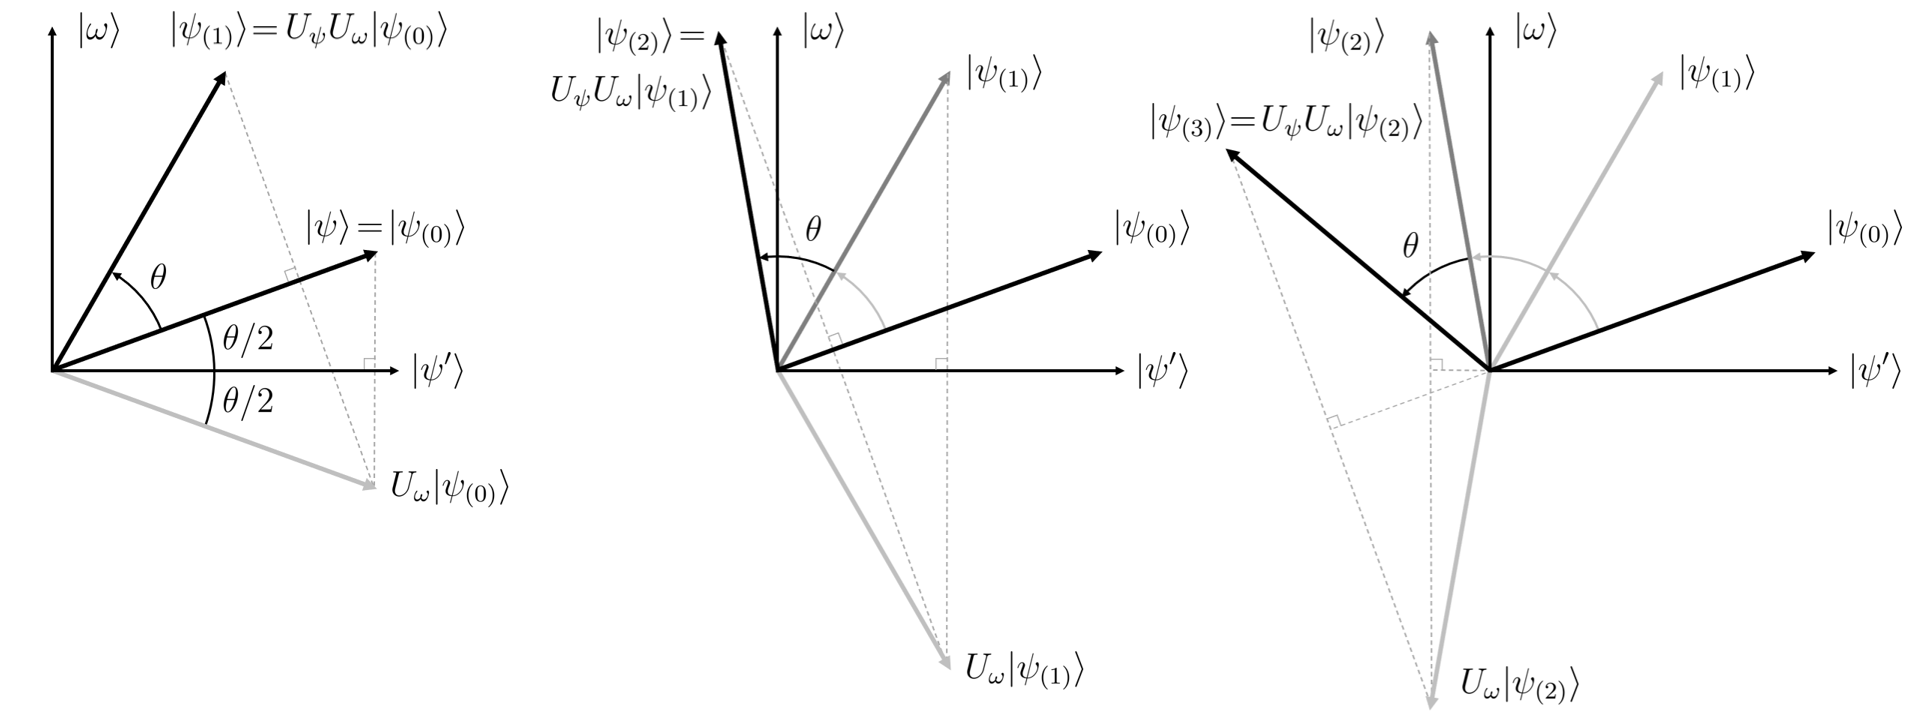
\includegraphics[scale=0.30]{GroverGeom.png}
\caption{Interprétation géométrique de l'algorithme de Grover}
\label{fig:GroverGeom}
\end{figure}
\noindent

\subsection{Préparation d'un q-échantillon}
\label{prepQE}
Pour exploiter les améliorations de complexité des algorithmes quantiques, il est nécessaire de pouvoir représenter un réseau bayésien par un circuit quantique. L'article de \cite{quant_rep_BN} propose une méthode pour générer des \textit{q-échantillons}, des vecteurs d'état représentant les échantillons de la distribution de probabilité du réseau bayésien.
\\
En bref, la préparation des q-échantillons s'effectue en trois principales étapes:
\begin{itemize}
    \item[1] Associer chaque variable du réseau bayésien à un ou plusieurs qubits (en fonction du nombre de valeurs prises par la variable).
    \item[2] Associer les probabilités (marginales ou conditionnelles) de chaque variable aux amplitudes des états composantes des qubits correspondants.
    \item[3] Encoder les amplitudes des états quantiques en utilisant des portes de rotation (contrôlées), dans un ordre topologique du graphe.
\end{itemize}
\noindent
Considérons d'abord un réseau bayésien composé de variables binaires. L'algorithme représente chaque variable par un qubit et effectue des rotations sur ces qubits pour leur attribuer la distribution de la table de probabilité conditionnelle (CPT) de la variable. Pour les racines du graphe, ce processus est directe, car la CPT a seulement deux entrées, correspondant aux états $|0\rangle$ et $|1\rangle$ d'un qubit. Pour les variables ayant des parents, il faut appliquer une série de rotations conditionnées par toutes les combinaisons de valeurs des parents. L'ordre des rotations est crucial, car les probabilités d'une variable dépendent de celles de ses parents; ainsi, les rotations doivent suivre un ordre topologique du graphe. 
\\
Pour les variables aléatoires discrètes pouvant prendre plusieurs valeurs, il faut binariser ces valeurs et utiliser plusieurs qubits pour représenter chaque variable. Les rotations sont plus complexes car elles impliquent plusieurs qubits. Il est donc nécessaire de procéder par étapes, en se concentrant sur un qubit à la fois. L'approche consiste à s'inspirer des rotations appliquées aux variables ayant des parents pour effectuer une binarisation de la variable discrète.
\\
La réalisation concrète de cette étape nécessite l'utilisation d'une fonction indicatrice et d'une fonction de binarisation, dont les détails complets sont fournis en annexe. %3
\begin{figure}[H]
    \centering
\scalebox{.9}{
\Qcircuit @C=1.0em @R=0.2em @!R { \\
	 	\lstick{{0} :  } & \qw \barrier[0em]{2} & \qw & \qw & \gate{\mathrm{R_Y}\,(\mathrm{1.772})} & \qw \barrier[0em]{2} & \qw & \gate{\mathrm{R_Y}\,(\mathrm{2.941})} \barrier[0em]{2} & \qw & \gate{\mathrm{X}} & \ctrl{1} & \gate{\mathrm{X}} \barrier[0em]{2} & \qw & \qw
   \\
	 	\lstick{{1} :  } & \gate{\mathrm{R_Y}\,(\mathrm{2.214})} & \qw & \gate{\mathrm{X}} & \ctrl{-1} & \gate{\mathrm{X}} & \qw & \ctrl{-1} & \qw & \gate{\mathrm{X}} & \ctrl{1} & \gate{\mathrm{X}} & \qw & \qw
   \\
	 	\lstick{{2} :  } & \qw & \qw & \qw & \qw & \qw & \qw & \qw & \qw & \qw & \gate{\mathrm{R_Y}\,(\mathrm{\pi})} & \qw & \qw & \qw
   \\
	 	\lstick{\mathrm{{meas} :  }} & \lstick{/_{_{3}}} \cw & \cw & \cw & \cw & \cw & \cw & \cw & \cw & \cw & \cw & \cw & \cw & \cw
   \\
\\ }
}
\hspace{20pt}
\scalebox{.9}{
\Qcircuit @C=.6em @R=0.2em @!R { \\
	 	\lstick{{0} :  } & \qw & \qw & \ctrl{1} & \qw \barrier[0em]{2} & \qw & \gate{\mathrm{X}} & \ctrl{1} & \gate{\mathrm{X}} \barrier[0em]{2} & \qw & \ctrl{1} \barrier[0em]{2} & \qw & \meter & \qw & \qw & \qw & \qw
   \\
	 	\lstick{{1} :  } & \qw & \gate{\mathrm{X}} & \ctrl{1} & \gate{\mathrm{X}} & \qw & \qw & \ctrl{1} & \qw & \qw & \ctrl{1} & \qw & \qw & \meter & \qw & \qw & \qw
   \\
	 	\lstick{{2} :  } & \qw & \qw & \gate{\mathrm{R_Y}\,(\mathrm{0.9273})} & \qw & \qw & \qw & \gate{\mathrm{R_Y}\,(\mathrm{0.6435})} & \qw & \qw & \gate{\mathrm{R_Y}\,(\mathrm{0.2003})} & \qw & \qw & \qw & \meter & \qw & \qw
   \\
	 	\lstick{\mathrm{{meas} :  }} & \cw & \cw & \cw & \cw & \cw & \cw & \cw & \cw & \cw & \cw & \cw & \dstick{_{_{\hspace{0.0em}0}}} \cw \ar @{<=} [-3,0] & \dstick{_{_{\hspace{0.0em}1}}} \cw \ar @{<=} [-2,0] & \dstick{_{_{\hspace{0.0em}2}}} \cw \ar @{<=} [-1,0] & \cw & \cw
   \\
\\ }
}

    \caption{Circuit quantique préparateur des q-échantillons du réseau bayésien de la figure \ref{fig:ExBN}}
    \label{fig:quantCirc}
\end{figure}

\noindent
Soit $\mathcal{B} = (G, \mathcal{X})$ un réseau bayésien, avec $\mathcal{X} = (X_i)_{i \in [\![1,k]\!]}$ une famille de variables aléatoires discrètes. Posons $N_i = |X_i(\Omega)|$, le nombre de valeurs prises par la variable $X_i$. Cette construction utilise $2^{\lceil \log_2(N_i) \rceil} - 1$ portes $C^nRY$ et $2^{\lceil \log_2(N_i) \rceil} - 2$ portes $C^nNOT$. Le nombre total de portes quantiques utilisées est donc majoré par :
\[\sum_{\substack{X_i \in \mathcal{X} \\ N_i = |X_i(\Omega)|}}
\left[
2^{\lceil \mathrm{log}_2(N_i)\rceil+1} \prod_{\substack{X_j\in Pa(X_i) \\ N_j = |X_j(\Omega)|}}N_j 
\right] 
\]
En particulier, pour un réseau bayésien  binaire à $k$ variables, posons $m = \underset{X_i \in \mathcal{X}}{\mathrm{max}}(|Pa(X_i)|)$, le degré entrant maximal. La complexité, calculée en nombre de portes quantiques, est de $\mathcal{O}(k2^m)$.

\subsection{Échantillonage quantique par la méthode de rejet}

Nous abordons maintenant le cœur du sujet : la partie mettant en œuvre l'ensemble des algorithmes étudiés jusqu'à présent. La construction que nous allons présenter ici s'appuie sur l'article de \cite{low2014quantum}.
\\
À partir des q-échantillons obtenus via la section précédente, nous utilisons l'amplification d'amplitude afin de réaliser l'inférence par la méthode de rejet. En effet, l'échantillonnage par rejet peut être perçu comme une recherche non structurée d'échantillons dans la distribution du réseau bayésien. L'amplification d'amplitude permet alors une amélioration de cette recherche par un facteur de racine carrée. Cette approche exploite les atouts de l'algorithme d'amplification d'amplitude pour augmenter la probabilité de sélection des échantillons pertinents, rendant le processus d'inférence plus efficace par rapport aux méthodes classiques.
\\
Encore une fois, dû aux contraintes de brièveté, nous invitons le lecteur à une étude détaillée en annexe. %4

\begin{algorithm}
\caption{Échantillonage quantique par la méthode de rejet}\label{alg:quant}
\vspace{8pt}
Soit $i$ l'itérateur de la boucle externe:
\begin{itemize}
    \item[1] Initialiser $|\psi \rangle = A|0\rangle^{\otimes k}$.
    \item[2] Appliquer l'itération de Grover $2^i$ fois:
    \item[] Pour $j \in [\![0, 2^i-1]\!]$,
    \begin{itemize}
  	    \item[2.1] Appliquer à $|\psi_{(j)}\rangle$ l'opérateur
   	    $
   	    U_{e} = Id_{\mathcal{Q}} \otimes (Id_{\mathcal{E}} -  2|e \rangle \langle e| )
   	    $
   	    \item[2.2] Appliquer à $|\psi_{(j)}\rangle$ l'opérateur
    	$
   	    U_{\psi} = 2|\psi\rangle \langle \psi | - Id_{\mathcal{H}}
   	    $
        \item[]Celui-ci est aussi donnée par 
    	$
    	U_{\psi} = AU_{0}A^{-1}
   	    $
    	où $U_{0} = 2|0\rangle \langle 0|^{\otimes k} - Id_{\mathcal{H}}$.
    \end{itemize}
    \item[] On se retrouve donc avec $|\psi_{(i+1)}\rangle = AU_{0}A^{-1}U_{e} |\psi_{(i)} \rangle$.
    \item[3] Mesurer les qubits d'observation $\mathcal{E}$ de l'état résultant $|\psi_{(2^i)} \rangle$: Soit $t$ le résultat.
	\item[4]
	\begin{itemize}
   	 \item[4.1] Si $t=e$: Fin de l'algorithme.
   	 \item[4.2] Sinon: Retourner à l'étape 1 en incrémentant $i$ de $1$.
    \end{itemize}
\end{itemize}
\end{algorithm}

\begin{figure}[H]
    \centering
\scalebox{1.0}{
\Qcircuit @C=.6em @R=.6em { \\
	 	\lstick{{\ket{0}} :  } & \multigate{2}{\mathrm{A}} & \multigate{2}{\mathrm{G^{2^i}}} & \meter & \qw & \qw & \qw \\
        \lstick{\raisebox{0.5em}{\vdots}\hspace{0.7em}} & \nghost{\mathrm{A}} & \nghost{\mathrm{G^{2^i}}} & & \raisebox{0.5em}{\rotatebox{35}{\vdots}} & & \\
        \lstick{{\ket{0}} :  } & \ghost{\mathrm{A}} & \ghost{\mathrm{G^{2^i}}} & \qw & \qw & \meter & \qw\\
	 	\lstick{\mathrm{{meas} :  }} & \cw & \lstick{/_{_{n}}} \cw & \dstick{_{_{\hspace{0.0em}1}}} \cw \ar @{<=} [-3,0] & \dstick{_{_{\hspace{0.0em}\hdots}}} \cw & \dstick{_{_{\hspace{0.0em}n}}} \cw \ar @{<=} [-1,0] & \cw\\
\\ }}
\caption{Circuit quantique d'une itération de la boucle externe de l'algorithme \ref{alg:quant}}
    \label{fig:GroverCirc}
\end{figure}

\noindent
Pour simplifier les notations, supposons que le réseau bayésien est composé de $k$ états binaires, avec $\mathcal{E}$ l'ensemble des états d'observation et $\mathcal{Q}$ les états cibles.
Soient $(e_i)_{i \in [\![1,|\mathcal{E}|]\!]}$ les qubits représentant les éléments de $\mathcal{E}$ et $e = e_1e_2\cdots e_{|\mathcal{E}|}$ la chaîne de bits correspondante. De la même manière définissons $q$ la chaîne représentant $\mathcal{Q}$.
Le but de l'algorithme est ainsi d'échantillonner à partir de la distribution $\mathbb{P}(\mathcal{Q}|\mathcal{E}=e)$.
\\
Soit $A$ l'opérateur unitaire qui prépare le q-échantillon $| \psi \rangle = A |0\rangle ^{\otimes k}$ (c.f. section \ref{prepQE}). En permutant les états de $\mathcal{E}$ à droite, on a une décomposition du q-échantillons avec des états contenant des observations correctes et incorrectes:
\\
Le système quantique est partitionné en deux espaces vectoriels orthogonaux : $\mathcal{H} = \mathcal{Q} \otimes (\mathcal{E}_0 \oplus \mathcal{E}_1)$, où $\mathcal{Q} \otimes \mathcal{E}_0$ contient les q-échantillons de la distribution $\mathbb{P}(\mathcal{Q,E}|\mathcal{E}\neq e)$, et $\mathcal{Q} \otimes \mathcal{E}_1$ de $\mathbb{P}(\mathcal{Q,E}|\mathcal{E} = e)$. En appliquant l'amplification d'amplitude, on obtient un q-échantillon de la distribution $\mathbb{P}(\mathcal{Q}|\mathcal{E} = e)$ avec haute probabilité. 
\begin{figure}[H]
    \centering
\scalebox{.8}{
\raisebox{-1em}{
\Qcircuit @C=.6em @R=.6em { \\
	 	\qw & \multigate{2}{\mathrm{G}} & \qw \\
        \raisebox{0.5em}{\vdots} & \nghost{\mathrm{G}} & \raisebox{0.5em}{\vdots} \\
        \qw & \ghost{\mathrm{G}} & \qw \\
\\ }
\hspace{0.5em}
\raisebox{-2.9em}{\Large =}
\hspace{0.5em}
\Qcircuit @C=.6em @R=.6em { \\
	 	\qw & \multigate{2}{\mathrm{U_e}} & \multigate{2}{\mathrm{A^{\dag}}} & \multigate{2}{\mathrm{U_0}} & \multigate{2}{\mathrm{A}} & \qw \\
        \raisebox{0.5em}{\vdots} & \nghost{\mathrm{U_e}} & \nghost{\mathrm{A^{\dag}}} & \nghost{\mathrm{U_0}} & \nghost{\mathrm{A}} & \raisebox{0.5em}{\vdots} \\
        \qw & \ghost{\mathrm{U_e}} & \ghost{\mathrm{A^{\dag}}} & \ghost{\mathrm{U_0}} & \ghost{\mathrm{A}} & \qw \\
\\ }
}

\hspace{3em}

\raisebox{-0.8em}{
\Qcircuit @C=.6em @R=.8em { \\
	 	\qw & \multigate{2}{\mathrm{U_e}} & \qw \\
        \raisebox{0.5em}{\vdots} & \nghost{\mathrm{U_e}} & \raisebox{0.5em}{\vdots} \\
        \qw & \ghost{\mathrm{U_e}} & \qw \\
\\ }
}

\hspace{0.5em}
\raisebox{-4.1em}{\Large =}
\hspace{1em}

\Qcircuit @C=.6em @R=1em {
\lstick{} & \qw & \qw & \qw & \qw \\
\lstick{} & \raisebox{0.5em}{\vdots} & & \raisebox{0.5em}{\vdots} & \\
\lstick{} & \qw & \qw & \qw & \qw 
\inputgroupv{1}{3}{.8em}{1.4em}{\mathcal{Q}}\\
\lstick{} & \gate{\mathrm{X_{1}^{1-e_1}}} & \ctrl{2} & \gate{\mathrm{X_{1}^{1-e_1}}} & \qw \\
\lstick{} & \raisebox{0.5em}{\vdots} & & \raisebox{0.5em}{\vdots} & \\
\lstick{} & \gate{\mathrm{X_{\scalebox{.7}{$|\mathcal{E}|$}}^{1-e_{\scalebox{.5}{$|\mathcal{E}|$}}}}} & \control\qw & \gate{\mathrm{X_{\scalebox{.7}{$|\mathcal{E}|$}}^{1-e_{\scalebox{.5}{$|\mathcal{E}|$}}}}} & \qw \\
\inputgroupv{4}{6}{0.8em}{2.4em}{\mathcal{E}}\\
}
}
\caption{Circuit des portes quantiques utilisées dans \ref{fig:GroverCirc}}
    \label{fig:GatesCirc}
\end{figure}
\noindent
L'amplification d'amplitude effectue des rotations sur le q-échantillon pour l'orienter vers le sous-espace vectoriel $\mathcal{E}_1$, contenant les bonnes observations. Ainsi, la mesure produit un échantillon pertinent avec une haute probabilité. En se basant sur la section \ref{prepQE}, la complexité totale en espérance pour générer un échantillon de la distribution $\mathbb{P}(\mathcal{Q}|\mathcal{E}=e)$ est de $\mathcal{O}(k2^m/\sqrt{P_e})$. La préparation de q-échantillons et l'itération de Grover prennent $\mathcal{O}(k2^m)$, et en moyenne, ces opérations sont répétées $\mathcal{O}(1/\sqrt{P_e})$ fois, ce qui explique la complexité finale.